\documentclass[aspectratio=43]{beamer}
% Theme works only with a 4:3 aspect ratio
\usetheme{CSCS}

\usepackage{tikz}

\usepackage{pgfplots}
\usepackage{pgfplotstable}
\usetikzlibrary{pgfplots.groupplots,spy,patterns}
\usetikzlibrary{arrows.meta}
\usetikzlibrary{positioning}
\usepackage{listings}
\usepackage{color}
\usepackage{dirtree}
\usepackage{tcolorbox}
\usepackage{anyfontsize}
\usepackage{xspace}
\usepackage{graphicx}
\usepackage{pifont}

% define footer text
\newcommand{\footlinetext}{Alps User Environments}

% Select the image for the title page
\newcommand{\picturetitle}{slide-images/image5.pdf}

% fonts for maths
\usefonttheme{professionalfonts}
%\usefonttheme{serif}

\definecolor{codegreen}{rgb}{0,0.6,0}
\definecolor{codegray}{rgb}{0.5,0.5,0.5}
\definecolor{codepurple}{rgb}{0.58,0,0.82}
\definecolor{backcolour}{rgb}{0.95,0.95,0.95}

\lstdefinestyle{defaultstyle}{
    backgroundcolor=\color{backcolour},
    commentstyle=\color{codegreen},
    keywordstyle=\color{magenta},
    stringstyle=\color{codepurple},
    basicstyle=\ttfamily\footnotesize,
    breakatwhitespace=false,
    breaklines=true,
    captionpos=b,
    keepspaces=true,
    showspaces=false,
    showstringspaces=false,
    showtabs=false,
    tabsize=2
}

\lstset{style=defaultstyle}

\newcommand\YAMLcolonstyle{\ttfamily\color{magenta}\bfseries\footnotesize}
\newcommand\YAMLkeystyle{\ttfamily\color{blue!50!black}\bfseries\footnotesize}
\newcommand\YAMLvaluestyle{\ttfamily\color{green!50!black}\bfseries\footnotesize}

\makeatletter

% here is a macro expanding to the name of the language
% (handy if you decide to change it further down the road)
\newcommand\language@yaml{yaml}

\expandafter\expandafter\expandafter\lstdefinelanguage
\expandafter{\language@yaml}
{
  keywords={true,false,null,y,n},
  keywordstyle=\color{darkgray}\bfseries,
  basicstyle=\YAMLkeystyle,                                 % assuming a key comes first
  sensitive=false,
  comment=[l]{\#},
  morecomment=[s]{/*}{*/},
%  commentstyle=\color{purple}\ttfamily,
%  stringstyle=\YAMLvaluestyle\ttfamily,
  moredelim=[l][\color{orange}]{\&},
  moredelim=[l][\color{magenta}]{*},
  moredelim=**[il][\YAMLcolonstyle{:}\YAMLvaluestyle]{:},   % switch to value style at :
  morestring=[b]',
  morestring=[b]",
  literate =    {---}{{\ProcessThreeDashes}}3
                {>}{{\textcolor{red}\textgreater}}1     
                {|}{{\textcolor{red}\textbar}}1 
                {\ -\ }{{\mdseries\ -\ }}3,
}

% hyperlink formatting
\hypersetup{
    unicode=true,          % non-Latin characters in Acrobat’s bookmarks
    colorlinks=true,       % colored links
    linkcolor=blue,
    urlcolor=blue
}


% source code listing
\newcommand\TS{\rule{0pt}{2.6ex}}       % Top strut
\newcommand\BS{\rule[-1.2ex]{0pt}{0pt}} % Bottom strut
\newcommand{\hl}[1]{\textbf{\textcolor{blue}{#1}}} % for hilighting optimal entries in tables
\newcommand{\rl}[1]{\textbf{\textcolor{red}{#1}}} % for hilighting sub-optimal entries in tables
\newcommand{\img}[1]{{\Large \textbf{IMAGE {#1}}}}
\newcommand{\hilight}[1]{\textcolor{blue!20!orange}{#1}}
\newcommand{\alps}[0]{Alps\xspace}
\newcommand{\stackinator}[0]{Stackinator\xspace}
\newcommand{\stackboxwidth}[0]{5cm}
\newcommand{\stackboxheight}[0]{1cm}
\newcommand{\stacksystemcolor}[0]{blue!10}
\newcommand{\stackbootstrapcolor}[0]{green!10}
\newcommand{\stackcolor}[0]{orange!10}

% set indent to a more reasonable level (so that itemize can be used in columns)
\setlength{\leftmargini}{20pt}

\DeclareTextFontCommand{\emph}{\color{blue!85!black}}

\author{
    \textbf{B.~Cumming},
    J.~Coles,
    T-I.~Manitaras,
    J-G.~Piccinali,
    S.~Pintarelli,
    H.~Stoppels}
\title{\centering Deploying Alternative User Environments on Alps}
\subtitle{CUG23 -- Helsinki}

\begin{document}

\setlength\labelsep   {\dimexpr\labelsep - 0.2em\relax}
\setlength\leftmargini{\dimexpr\leftmargini - 1.0em\relax}

% TITLE SLIDE
\cscstitle

%-------------------------------------------
\begin{frame}[fragile]{}
    \vspace{-60pt}
    \begin{center}
    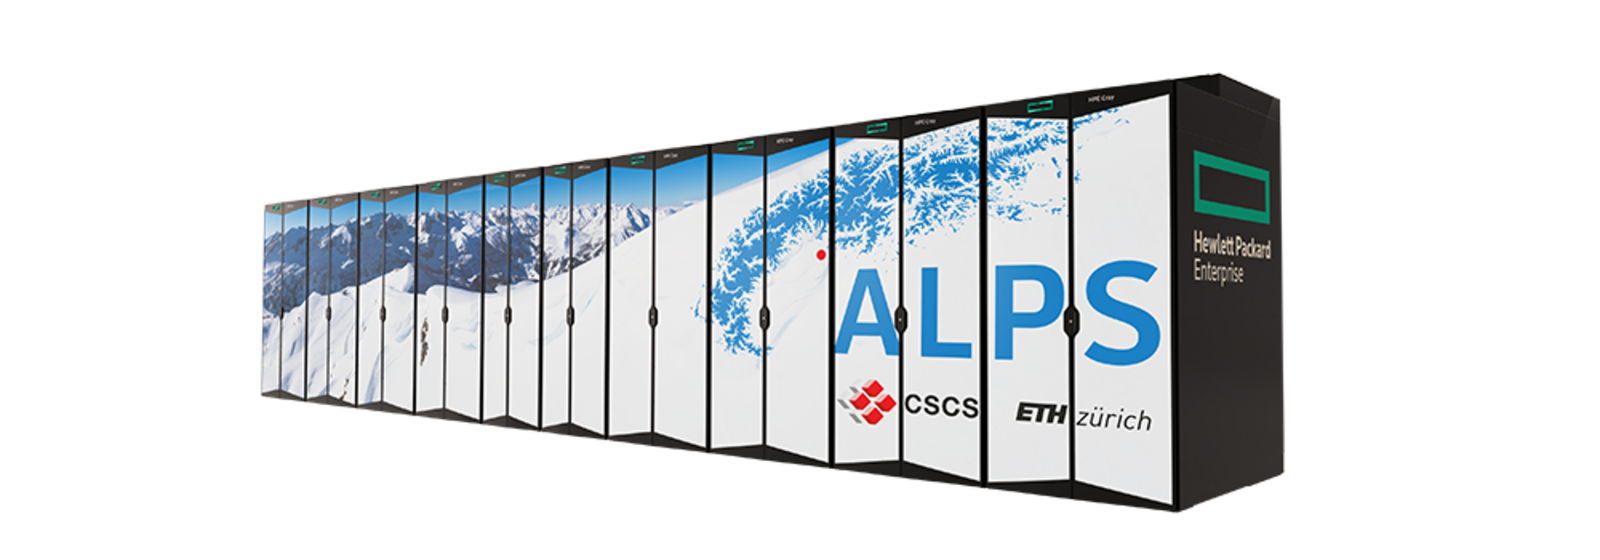
\includegraphics[width=\textwidth]{images/alps.png}

    Alps is the new HPE Cray EX-based infrastructure at CSCS.

    \vspace{15pt}

        Consolidate separate service-specific clusters onto a single infrastructure -- versatile software-defined clusters (\emph{vClusters}) with workload-specific software environment, scheduler, storage and network isolation.

    \vspace{15pt}

    \dots software stack deployment won't scale with our existing deployment model\dots

    \end{center}

\end{frame}
%-------------------------------------------

%-------------------------------------------
\begin{frame}[fragile]{Monolithic Software Stacks}
    \begin{columns}[T]
        \begin{column}{0.5\textwidth}
            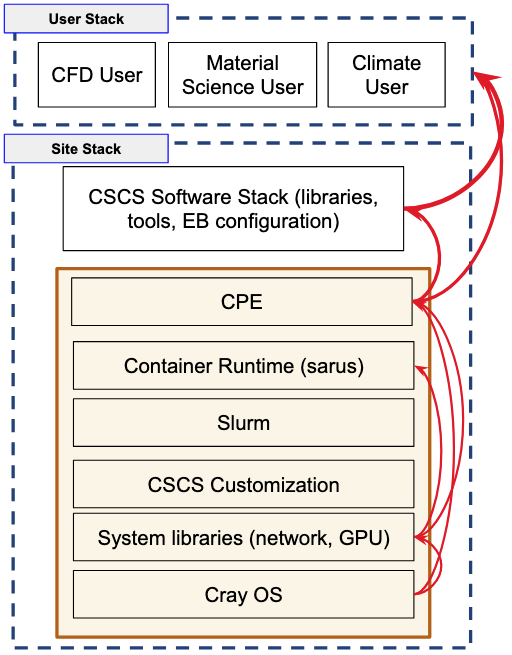
\includegraphics[width=\textwidth]{images/stack-old.png}
        \end{column}
        \begin{column}{0.5\textwidth}

            \small

            Sites provide CPE -- then provide software built on top:
            % point out presentations past and present
            \begin{itemize}
                \item install \emph{all the software for all the users} on a shared file system;
                \item use CPE modules + site modules for environment customisation.
            \end{itemize}

            CPE presents challenges as a software stack foundation:
            \begin{itemize}
                \item changes every 3 months 
                \item has a large surface area of possible bugs and regressions.
                \item deploying fixes takes minimum 3-6 months.
            \end{itemize}
        \end{column}
    \end{columns}
\end{frame}
%-------------------------------------------

%-------------------------------------------
\begin{frame}[fragile]{Bespoke SW stacks}
    \begin{columns}[T]
        \begin{column}{0.6\textwidth}
            Start with a simpler foundation:
            \begin{itemize}
                \item CrayOS + libfabric + Slurm;
                \item no CPE;
                \item less frequent changes over a smaller area.
            \end{itemize}

            Provide workflow-specific software stacks:
            \begin{itemize}
                \item only the packages that are needed;
                \item deployed independently;
                \item built using Spack.
            \end{itemize}

            \begin{center}
            \emph{``You can create environments without modules using Spack. ''}\\
            \emph{``It is tricky to configure Spack. ''}
            \end{center}


        \end{column}
        \begin{column}{0.5\textwidth}
            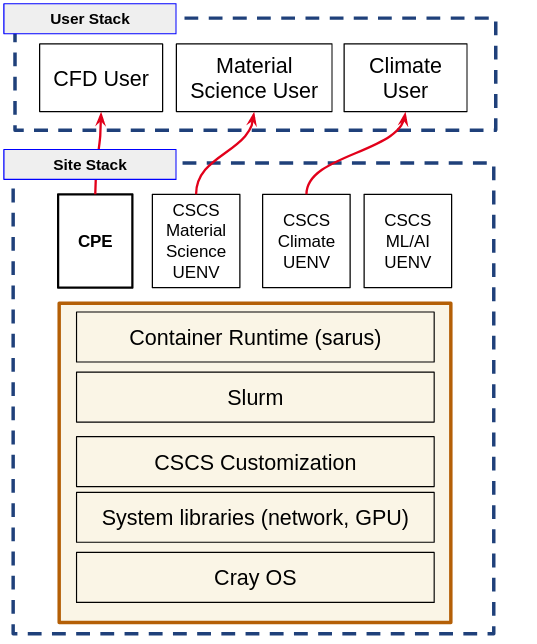
\includegraphics[width=\textwidth]{images/stack-new.png}
        \end{column}
    \end{columns}
\end{frame}
%-------------------------------------------

\cscschapter{The Stackinator: Building Environments}

%-------------------------------------------
\begin{frame}[fragile]{Stackinator is Opinionated}
    \begin{center}
        Self contained software stacks are built through a workflow codified in a tool CSCS developed \emph{Stackinator}.

    \vspace{10pt}

        \textbf{provide the inputs}: \emph{YAML recipe} and \emph{system configuration} \dots

    \vspace{10pt}

        \textbf{perform the steps}: \emph{stack-config} then \emph{make} \dots

    \vspace{10pt}

        \dots to build a software stack following the best-practices and HPE Cray EX-specific methods developed by CSCS (Harmen Stoppels).

    \vspace{10pt}

        \emph{Each stack exposes a spack upstream interface, and optional modules and environment views.}

    \end{center}

    \url{https://github.com/eth-cscs/stackinator}
\end{frame}
%-------------------------------------------

%-------------------------------------------
\begin{frame}[fragile]{Stackinator}
    Stackinator provides a CLI tool to configure the software stack on the target system:

            \begin{lstlisting}[style=talkbash]
> stack-config --recipe $recipe_path \
    --system $CLUSTERNAME --build /dev/shm/build
> cd /dev/shm/build
> env --ignore-environment PATH=/usr/bin:/bin:`pwd`/spack/bin make store.squashfs -j64
            \end{lstlisting}

    \begin{itemize}
        \item \emph{recipe}: YAML files that describe compilers, software packages, and tests for software stack.
        \item \emph{system}: System config for few libraries (gcc, libfabric, xpmem, slurm, rdma-core).
        \item \emph{mount}: The installation path (in the recipe).
        \item \emph{build}: Where the build will be performed.
    \end{itemize}
\end{frame}

%-------------------------------------------
\begin{frame}[fragile]{Stacks}
    A ``Spack Stack'' is built in layers on top of a handful of external system dependencies.
    \begin{center}
        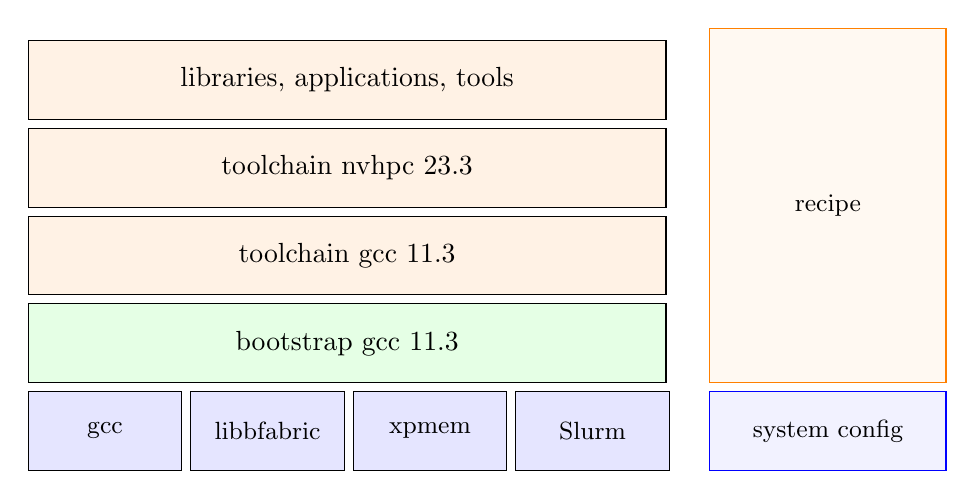
\begin{tikzpicture}
    \node[rectangle, draw=black, fill=\stacksystemcolor, minimum width=1.95cm, minimum height=1cm]
        (system_gcc) {\small gcc};
    \node[rectangle, draw=black, fill=\stacksystemcolor, minimum width=1.95cm, minimum height=1cm,
        right=0.1cm of system_gcc]
        (libfabric) {\small libbfabric};
    \node[rectangle, draw=black, fill=\stacksystemcolor, minimum width=1.95cm, minimum height=1cm,
        right=0.1cm of libfabric]
        (xpmem) {\small xpmem};
    \node[rectangle, draw=black, fill=\stacksystemcolor, minimum width=1.95cm, minimum height=1cm,
        right=0.1cm of xpmem]
        (slurm) {\small Slurm};
    \node[rectangle, draw=blue, fill=blue!5, minimum width=3cm, minimum height=1cm,
        right=0.5cm of slurm]
        (sysconfig) {\small system config};
    \node[rectangle, draw=black, fill=\stackbootstrapcolor, minimum width=8.1cm, minimum height=1cm,
        above=0.1cm of system_gcc.north west, anchor=south west]
        (bootstrap) {bootstrap gcc 11.3};
    \node[rectangle, draw=orange, fill=orange!5, minimum width=3cm, minimum height=4.5cm,
        above=0.1cm of sysconfig]
        (slurm) {\small recipe};
    \node[rectangle, draw=black, fill=\stackcolor, minimum width=8.1cm, minimum height=1cm,
        above=0.1cm of bootstrap]
        (gcc) {toolchain gcc 11.3};
    \node[rectangle, draw=black, fill=\stackcolor, minimum width=8.1cm, minimum height=1cm,
        above=0.1cm of gcc]
        (nvhpc) {toolchain nvhpc 23.3};
    \node[rectangle, draw=black, fill=\stackcolor, minimum width=8.1cm, minimum height=1cm,
        above=0.1cm of nvhpc]
        (software) {libraries, applications, tools};
   %\node[rectangle, draw=black, fill=\stackcolor, minimum width=4cm, minimum height=1.5cm,
   %    above=0.1cm of nvhpc.north west, anchor=south west]
   %    (env-gnu) {prgenv-gnu};
   %\node[rectangle, draw=black, fill=\stackcolor, minimum width=4cm, minimum height=1.5cm,
   %    right=0.1cm of env-gnu]
   %    (env-openacc) {prgenv-openacc};
\end{tikzpicture}


    \end{center}
\end{frame}
%-------------------------------------------


%-------------------------------------------
\begin{frame}[fragile]{System Configurations}
    A Spack configuration for the target vCluster that describes the handful of system dependencies.

    \begin{columns}[T]
        \begin{column}{0.5\textwidth}
        \begin{codecolumn}{compilers.yaml}
            \begin{lstlisting}[style=talkyaml]
compilers:
- compiler:
 spec: gcc@7.5.0
  paths:
   cc: /usr/bin/gcc
   cxx: /usr/bin/g++
   f77: /usr/bin/gfortran
   fc: /usr/bin/gfortran
  flags: {}
  operating_system: sles15
  target: x86_64
            \end{lstlisting}
        \end{codecolumn}
        \end{column}
        \begin{column}{0.5\textwidth}
        \begin{codecolumn}{packages.yaml}
            \begin{lstlisting}[style=talkyaml]
packages:
 libfabric:
  buildable: false
  externals:
  - spec: libfabric@1.15.2.0
    prefix: /opt/cray/libfabric/1.15.2.0/
 slurm:
  buildable: false
  externals:
  - spec: slurm@22-5-2
    prefix: /usr
 xpmem: ...
 rdma-core: ...
            \end{lstlisting}
        \end{codecolumn}
        \end{column}
    \end{columns}
\end{frame}

%-------------------------------------------
\begin{frame}[fragile]{Recipe: general configuration}

Name, mount point, the version of Spack to use and mirror configuration.

\begin{code}{\lstinline{config.yaml}}
\lstinputlisting[style=talkyaml]{src/nv-recipe/config.yaml}
\end{code}

\end{frame}
%-------------------------------------------

%-------------------------------------------
\begin{frame}[fragile]{Recipe: compiler toolchains}

Compilers are built in three stages
\begin{enumerate}
\item \emph{bootstrap}: gcc built using the system compiler (gcc 7.5.0).
%    * `gcc:specs`: single spec of the form `gcc@version`.
%    * no Fortran, not optimised
%    * The selected version should have full support for the target architecture in order to build optimised gcc toolchains in step 2.
%    * tabes 2.5 minutes to build
\item \emph{gcc}: Optimised gcc version(s) provided by the stack.
%    * `gcc:specs`: A list of _at least one_ of the specs of the form `gcc@version`.
%    * includes Fortran, tuned.
%    * takes 25 minutes to build
\item \emph{llvm}: (optional) nvhpc and/or llvm toolchains buil with gcc from step 2.
%    * `llvm:specs`: a list of specs of the form `nvhpc@version` or `llvm@version`.
%    * `llvm:requires`: the version of gcc from step 2 that is used to build the llvm compilers.
\end{enumerate}


\begin{code}{\lstinline{compilers.yaml}}
\lstinputlisting[style=talkyaml]{src/nv-recipe/compilers-annotated.yaml}
\end{code}

\end{frame}
%-------------------------------------------

%-------------------------------------------
\begin{frame}[fragile]{Recipe: environments}

    \begin{columns}[T]
        \begin{column}{0.5\textwidth}
        \begin{codecolumn}{environments.yaml}
\lstinputlisting[style=talkyaml, firstline=1, lastline=16]{src/nv-recipe/environments.yaml}
        \end{codecolumn}
        \end{column}
        \begin{column}{0.5\textwidth}
        \begin{codecolumnnotitle}{}
\lstinputlisting[style=talkyaml, firstline=17]{src/nv-recipe/environments.yaml}
        \end{codecolumnnotitle}
        \end{column}
    \end{columns}

\end{frame}
%-------------------------------------------

%-------------------------------------------
\begin{frame}[fragile]{Building}
    \begin{columns}[T]
        \begin{column}{0.6\textwidth}
            stack-config generates a build path with a hierarchy of Makefiles that build the stack as a DAG of Spack environments.
            \begin{itemize}
                \item build path is in /dev/shm -- build in memory
                \item Bubblewrap (bwrap) is used to mount the \emph{store} path at the destination during builds
            \end{itemize}
            %\begin{center}
                \hspace{1.5cm}\begin{tikzpicture}[node distance=1cm and 2.75cm,
    transform canvas={scale=0.7},
            nodes={draw, rectangle, rounded corners, minimum height=0.5cm, minimum width=3cm, fill=blue!10, inner sep=0.3cm},
            arrows={-Stealth}]
    % Nodes
    \node[] (bootstrap) {bootstrap};
    \node[below=of bootstrap] (gcc) {gcc};
    \node[right=of gcc] (llvm) {llvm};
    \node[fill=green!15, below=of gcc] (prgenv-gcc) {prgenv-gcc};
    \node[fill=green!15, right=of prgenv-gcc] (prgenv-openacc) {prgenv-openacc};

    % Edges
    \draw (bootstrap)
        edge node[midway, fill=white,rectangle,fill=red!5, draw=red, inner sep=0.1cm, minimum height=0.3cm, minimum width=1 cm]
        {\scriptsize gcc@11\%gcc@7.5}
        (gcc);
    \draw (gcc) 
        edge node[midway, fill=white,rectangle,fill=red!5, draw=red, inner sep=0.1cm, minimum height=0.3cm, minimum width=1 cm]
        {\scriptsize gcc@11\%gcc@11}
        (llvm);
    \draw (gcc) 
        edge node[midway, fill=white,rectangle,fill=red!5, draw=red, inner sep=0.1cm, minimum height=0.3cm, minimum width=1 cm]
        {\scriptsize gcc@11\%gcc@11}
        (prgenv-gcc);
    \draw (gcc) 
        edge node[midway, fill=white,rectangle,fill=red!5, draw=red, inner sep=0.1cm, minimum height=0.3cm, minimum width=1 cm]
        {\scriptsize gcc@11\%gcc@11}
        (prgenv-openacc);
    \draw (llvm) 
        edge node[midway, fill=white,rectangle,fill=red!5, draw=red, inner sep=0.1cm, minimum height=0.3cm, minimum width=1 cm]
        {\scriptsize nvhpc@22.7\%gcc@11}
        (prgenv-openacc);
\end{tikzpicture}

            %\end{center}
        \end{column}


        \begin{column}{0.4\textwidth}
            {
            \setlength{\DTbaselineskip}{5pt}
            \footnotesize
            \dirtree{%
.1 /dev/shm/nvidia-build.
.2 Makefile.
.2 spack.
.2 compilers.
.3 Makefile.
.3 bootstrap.
.4 spack.yaml.
.4 \textcolor{blue}{compilers.yaml}.
.4 \textcolor{blue}{packages.yaml}.
.4 \textcolor{blue}{Makefile}.
.3 gcc.
.4 spack.yaml.
.3 llvm.
.4 spack.yaml.
.2 environments.
.3 Makefile.
.3 gcc-env.
.4 spack.yaml.
.3 nvhpc-env.
.4 spack.yaml.
.2 store.
}


            }
        \end{column}
    \end{columns}
\end{frame}
%-------------------------------------------

%-------------------------------------------
\begin{frame}[fragile]{Wait! What about MPI?}
    \begin{columns}[T]
        \begin{column}{0.65\textwidth}
            Cray-mpich is the only robust MPI for SS11 as of May 2023.
            \begin{itemize}
                \item We used OpenMPI+ucx on SS10
            \end{itemize}
                % (early version of the stack used OpenMPI on SS10)
                % (OpenMPI and MPICH would be very welcome)

            \vspace{10pt}

            Stackinator uses a custom Spack package for cray-mpich:
            \begin{itemize}
                \item Repackage headers, libs, compiler wrappers from RPMs.
                \item Store as tar-balls CSCS-private artifactory.
                \item Run patchelf on libraries and string-substitution on compiler wrappers.
            \end{itemize}
            \emph{It takes an engineer an hour to create the binary package for each new CPE release.}
        \end{column}
        \hspace{-40pt}
        \begin{column}{0.4\textwidth}
            {
            \setlength{\DTbaselineskip}{5pt}
            \footnotesize
            \input{src/cray-mpich-tree-short.txt}
            }
        \end{column}
    \end{columns}

\end{frame}
%-------------------------------------------

%-------------------------------------------
\begin{frame}[fragile]{MPI Configuration is Opinionated}

\begin{code}{environments.yaml: "The user requests cray-mpich"}
    \begin{lstlisting}[style=talkyaml]
myenv:
    compiler:
    - toolchain: gcc
      spec: gcc@11
    mpi:
      spec: cray-mpich@8.1.18.4
      gpu: cuda \end{lstlisting}
\end{code}

\begin{code}{Generated Spack specs in spack.yaml}
    \begin{lstlisting}[style=talkyaml]
# cray-mpich specs are "simple"
specs:
- cray-mpich@8.1.18.4 +cuda

# The tool can generate more complex specs, e.g. OpenMPI on SS10:
specs:
- openmpi@4.0:4 +cuda +cxx +pmi schedulers=slurm fabrics=ucx
- ucx +rdmacm +cma +verbs +xpmem +ib_hw_tm +mlx5_dv +dc +ud +rc +dm +optimizations +gdrcopy ~assertions ~debug \end{lstlisting}
\end{code}

\end{frame}
%-------------------------------------------

%-------------------------------------------
\begin{frame}[fragile]{Spack package}

\begin{code}{repo/packages/cray-mpich/package.py}
    \begin{lstlisting}[style=talkbash]
@run_after("install")
def fixup_binaries(self):
  for root, _, files in os.walk(self.prefix):
    for f in [os.path.join(root, name) for name in files]
      if not self.should_patch(f): continue
      patchelf("--force-rpath", "--set-rpath", rpath, f)
      if "libmpi_gtl_cuda.so" in str(f):
        patchelf("--add-needed", "libstdc++.so", f)

@run_after("install")
def fixup_compiler_paths(self):
  filter("@@CC@@", self.compiler.cc,self.prefix.bin.mpicc)
  filter("@@PREFIX@@", self.prefix, self.prefix.bin.mpicc)
  if   "+cuda" in self.spec:gtl_library = "-lmpi_gtl_cuda"
  elif "+rocm" in self.spec:gtl_library = "-lmpi_gtl_hsa"
  else:                     gtl_library = ""
  filter("@@GTL@@", gtl_library, self.prefix.bin.mpicc) \end{lstlisting}
\end{code}

\end{frame}
%-------------------------------------------

%-------------------------------------------
\begin{frame}[fragile]{Optimising Build Times}
    Building stacks is resource intensive: 30~min -- 3~hours with 64-cores.

    \vspace{10pt}

    Build times are the main pain point for developers.

    \vspace{10pt}

    \begin{itemize}
        \item \emph{Parallelise the build}: build Spack environments in parallel
        \begin{itemize}
            \item Expose every opportunity to build packages concurrently.
        \end{itemize}
        \item \emph{Build in memory}:
        \begin{itemize}
            \item Build in /dev/shm.
            \item Use Bubblewrap (bwrap) to bind to the target installation path.
        \end{itemize}
        \item \emph{Cache previous builds}:
        \begin{itemize}
            \item Only build packages once.
            \item Use Spack binary build caches.
        \end{itemize}
    \end{itemize}
\end{frame}
%-------------------------------------------

%-------------------------------------------
\begin{frame}[fragile]{Optimising Build Times}
    \begin{center}
        \begin{tikzpicture}[scale=1]
    \begin{axis} [
        ymin = 0, ymax=3000,
        ybar, bar width = 18pt,
        %symbolic x coords={1,2,3,4},
        grid=major,
        xtick = {1,2,3,4},
        xticklabels = {scratch, memory, cache, partial},
        xticklabel style={text height=1ex},
        ylabel={Build time (s)},
        nodes near coords,
        nodes near coords style={fill=white},
    ]
        \addplot[fill=orange!30] table[x=id, y=time-s] {./data/stack-build.tbl};
        \draw[line width=2pt, ->] (axis cs:2,2714) -- (axis cs:2,1866);
        \draw[line width=2pt, ->] (axis cs:3,1566) -- (axis cs:3,445);
        \draw[line width=2pt, ->] (axis cs:4,1566) -- (axis cs:4,787);
        \node[fill=white] () at (axis cs:2,2300) {\bfseries 1.7x};
        \node[fill=white] () at (axis cs:3,1000) {\bfseries 10.8x};
        \node[fill=white] () at (axis cs:4,1200) {\bfseries 3.2x};

        %\draw (s1_t.center) -- (s1_b.center);
    \end{axis}
\end{tikzpicture}


    \end{center}
\end{frame}
%-------------------------------------------


\cscschapter{Deploying spack-stacks}

%-------------------------------------------
\begin{frame}[fragile]{SquashFS}
    The software stack can be copied to a shared file system once built.

    \vspace{20pt}

    At CSCS they are deployed as SquashFS images:
    \begin{itemize}
        \item consistent performance -- always faster than a shared file system;
        \item reduced storage requirements -- compression and deduplication.
        \item each stack is a single binary artifact -- easy to version, roll back and manage in CI/CD pipelines.
    \end{itemize}

    \vspace{20pt}

    \begin{center}
    \emph{SquashFS requires some additional tooling...}
    \end{center}
\end{frame}
%-------------------------------------------

%-------------------------------------------
\begin{frame}[fragile]{CLI Utilities}
    Non-privileged users are able to mount SquashFS images at runtime using the \emph{squashfs-mount} CLI setuid utility that:
    \begin{enumerate}
    \item creates a new mount namespace;
    \item mounts the SquashFS file through \emph{libmount};
    \item then drops privileges and executes a given command.
    \end{enumerate}

    \begin{code}{mounting a squashfs image}
\lstinputlisting[style=talkyaml]{src/squashfs-mount.sh}
    \end{code}

    \begin{center}
        \textbf{The image is mounted in the new process -- processes (users) on the same node can mount different images.}
    \end{center}

    \vspace{10pt}

    Open Source on GitHub with RPMs for Cray EX.\\\url{https://github.com/eth-cscs/squashfs-mount}
\end{frame}
%-------------------------------------------

%-------------------------------------------
\begin{frame}[fragile]{CLI Utilities}
    A CLI tool \emph{uenv} is under development.
    \begin{enumerate}
    \item for listing, starting, stopping user-environments
    \end{enumerate}

    \begin{code}{mounting a squashfs image}
\lstinputlisting[style=talkyaml]{src/uenv.sh}
    \end{code}

    \vspace{10pt}

    Open Source on GitHub.\\\url{https://github.com/eth-cscs/uenv}
\end{frame}
%-------------------------------------------

%-------------------------------------------
\begin{frame}[fragile]{SLURM}
    A Slurm plugin manages mounting environmnents on compute nodes.
    \begin{code}{Launch with explicit flags}
            \begin{lstlisting}[style=talkbash]
% srun --uenv-mount=/user-environment \
       --uenv-file=img.squashfs \
       -n2 -N2 osu_bw
            \end{lstlisting}
    \end{code}
    \begin{code}{Inherit the environment from the login node}
            \begin{lstlisting}[style=talkbash]
% squashfs-mount img.squashfs /user-environment bash
% srun -n2 -N2 osu_bw
            \end{lstlisting}
    \end{code}

    Also works intuitively for \emph{sbatch} -- user can set a default image that, and individual \emph{srun} in the script can use different environments.

    Open Source on GitHub with RPMs for Cray EX.\\\url{https://github.com/eth-cscs/slurm-uenv-mount/}
\end{frame}
%-------------------------------------------

%-------------------------------------------
\begin{frame}[fragile]{CI/CD}
    \begin{center}
    CI/CD pipelines \emph{from recipe to deployed SquashFS image} is a work in progress.
    \end{center}

    \vspace{10pt}

    Recipes are stored in a GitHub repository -- Pull requests and merges trigger a pipeline:
    \begin{enumerate}
        \item \emph{\sc Build Stage}: launch a Slurm job on the target cluster+architecture that uses stackinator to configure then build the image.
        \item push the generated image to a JFrog artifactory
        \item \emph{\sc Test Stage}: pull the image and run a Slurm job that executes ReFrame tests.
        \item post status to GitHub
        \item \emph{\sc Deploy Stage}: promote artifact to deployment artifactory (manual).
    \end{enumerate}

    \url{https://github.com/eth-cscs/alps-spack-stacks}
\end{frame}
%-------------------------------------------

\cscschapter{Results}

%-------------------------------------------
\begin{frame}[fragile]{OSU}
    We run OSU benchmarks compiled using CPE and Spack Stacks to understand the effect of packaging cray-mpich outside CPE.
\begin{center}
    \begin{tabular}{l |c  c }
                      & CPE   & Spack Stack \\
          \hline
        osu-benchmark & 5.9   & 5.9       \\
        cray-mpich    & 8.1.21& 8.1.24    \\
        gcc           & 11.2  & 11.3      \\
        cuda          & 11.6  & 11.8      \\
    \end{tabular}
\end{center}

    The benchmarks are run on \emph{Clariden}, a vCluster with \emph{64-core EPYC CPU} and  \emph{4 A100 GPUs} -- similar to Perlmutter.

\end{frame}
%-------------------------------------------

%-------------------------------------------
\begin{frame}[fragile]{OSU - P2P Bandwidth}
    \begin{center}
            \begin{tikzpicture}[scale=1]
        \begin{loglogaxis} [
            height=7cm, width=11cm,
            xmin = 1, xmax = 4194304,
            ymax = 40000, ymin=0.1,
            ytick={0.1,1,10,100,1000,10000},
            yticklabels={0.1,1,10,100,1000,10000},
            xtick={1,2,4,8,16,32,64,128,256,512,1024,2048,4096,8192, 16384,  32768,  65536,  131072, 262144, 524288, 1048576, 2097152, 4194304},
            xticklabels={1,2,4,8,16,32,64,128,256,512,1k,2k,4k,8k,16k,32k,64k,128k,256k,512k,1M,2M,4M},
            x tick label style={rotate=60,anchor=east},
            axis line style=very thick,
            ylabel=Bandwidth (MB/s),
            xlabel=Message Size,
            legend style = {at={(0.95,0.05)}, anchor=south east},
            grid=major
        ]
            \addplot[color=green!40!black,mark=square*,mark options={fill=white}, very thick]
                table[x=bytes, y=cpe-gpu-bw] {./data/osu/p2p.tbl};
            \addlegendentry{cpe/gpu}
            \addplot[color=orange!90!black,mark=*,mark options={fill=white}, very thick]
                table[x=bytes, y=sq-gpu-bw] {./data/osu/p2p.tbl};
            \addlegendentry{uenv/gpu}

            \addplot[color=blue!40!white,mark=square*,mark options={fill=white}, very thick]
                table[x=bytes, y=cpe-cpu-bw] {./data/osu/p2p.tbl};
            \addlegendentry{cpe/cpu}
            \addplot[color=yellow!70!black,mark=*,mark options={fill=white}, very thick]
                table[x=bytes, y=sq-cpu-bw] {./data/osu/p2p.tbl};
            \addlegendentry{uenv/cpu}

        \end{loglogaxis}
    \end{tikzpicture}

    \end{center}
\end{frame}
%-------------------------------------------

%-------------------------------------------
\begin{frame}[fragile]{OSU - P2P Latency}
    \begin{center}
            \begin{tikzpicture}[scale=1]
        \begin{loglogaxis} [
            height=7cm, width=11cm,
            xmin = 1, xmax = 4194304,
            ymax = 200, ymin=1,
            ytick={1,10,100},
            yticklabels={1,10,100},
            xtick={1,2,4,8,16,32,64,128,256,512,1024,2048,4096,8192, 16384,  32768,  65536,  131072, 262144, 524288, 1048576, 2097152, 4194304},
            xticklabels={1,2,4,8,16,32,64,128,256,512,1k,2k,4k,8k,16k,32k,64k,128k,256k,512k,1M,2M,4M},
            x tick label style={rotate=60,anchor=east},
            axis line style=very thick,
            ylabel=Latency ($\mu$s),
            xlabel=Message Size,
            legend style = {at={(0.05,0.95)}, anchor=north west},
            grid=major
        ]
            \addplot[color=green!40!black,mark=square*,mark options={fill=white}, very thick]
                table[x=bytes, y=cpe-gpu-lat] {./data/osu/p2p.tbl};
            \addlegendentry{cpe/gpu}
            \addplot[color=orange!90!black,mark=*,mark options={fill=white}, very thick]
                table[x=bytes, y=sq-gpu-lat] {./data/osu/p2p.tbl};
            \addlegendentry{uenv/gpu}

            \addplot[color=blue!40!white,mark=square*,mark options={fill=white}, very thick]
                table[x=bytes, y=cpe-cpu-lat] {./data/osu/p2p.tbl};
            \addlegendentry{cpe/cpu}
            \addplot[color=yellow!70!black,mark=*,mark options={fill=white}, very thick]
                table[x=bytes, y=sq-cpu-lat] {./data/osu/p2p.tbl};
            \addlegendentry{uenv/cpu}

        \end{loglogaxis}
    \end{tikzpicture}

    \end{center}
\end{frame}
%-------------------------------------------

%-------------------------------------------
\begin{frame}[fragile]{GROMACS}
    A GROMACS strong scaling benchmarks: a 1.4-million atom system (a pair of hEGFR Dimers of 1IVO and 1NQL) from the HECBioSim benchmarks suite.
\begin{center}
    \begin{tabular}{|l |c  c| }
        \cline{2-3}
\multicolumn{1}{c|}{} & CPE   & Spack Stack \\
        \hline
        gromacs       & 2021.5   & 2021.5   \\
        fftw          & 3.3.10   & 3.3.10   \\
        openblas      & 0.3.21   & 0.3.21   \\
        cray-mpich    & 8.1.21   & 8.1.24   \\
        gcc           & 11.2     & 11.3     \\
          \hline
    \end{tabular}
\end{center}

    Run on \emph{Clariden}, a vCluster with \emph{64-core EPYC CPU} and  \emph{4 Mi250x GPUs} -- identical to LUMI/Frontier/Setonix.
\end{frame}
%-------------------------------------------

%-------------------------------------------
\begin{frame}[fragile]{GROMACS - Strong Scaling}
    A difference of maximum $\pm$1.5\% between the CPE and the Spack-stack.
    \begin{center}
            \begin{tikzpicture}[scale=1]
        \begin{axis} [
            height=7cm, width=11cm,
            xmin = 1, xmax = 12,
            ymax = 40, ymin=0,
            ytick={5,10,15,20,25,30,35,40},
            %yticklabels={10,100,1000},
            xtick={1,2,3,4,5,6,7,8,9,10,11,12},
            xticklabels={1,2,3,4,5,6,7,8,9,10,11,12},
            %x tick label style={rotate=60,anchor=east},
            axis line style=very thick,
            ylabel=Throughput (ns/day),
            xlabel=Nodes,
            %title=\large \bf GROMACS through
            legend style = {at={(0.95,0.05)}, anchor=south east},
            grid=major
        ]
            \addplot[color=green!40!black,mark=square*,mark options={fill=white}, very thick]
                table[x=nodes, y=cpe-max] {./data/gromacs/hEGFRDimerPair.tbl};
            \addlegendentry{cpe}
            \addplot[color=orange!90!black,mark=*,mark options={fill=white}, very thick]
        table[x=nodes, y=uenv-max] {./data/gromacs/hEGFRDimerPair.tbl};
            \addlegendentry{uenv}
        \end{axis}
    \end{tikzpicture}


    \end{center}
\end{frame}
%-------------------------------------------

\cscschapter{Wrapping up}

%-------------------------------------------
\begin{frame}[fragile]{An opinionated appeal}
    \begin{center}
    Integration of other CPE products -- libsci, cce, etc -- would be great.

    \vspace{20pt}

    Spack support is simple:

    \vspace{20pt}

    \emph{CPE packages can be installed individually without environment variables or modules, like normal software}.

    \vspace{20pt}

    \emph{In an ideal world we could build cray-mpich and libfabric+CXI from source}.
    \end{center}
\end{frame}
%-------------------------------------------

\cscschapter{Thank you}

\cscschapter{Backup}

%-------------------------------------------
\begin{frame}[fragile]{DDT}
    \begin{center}
        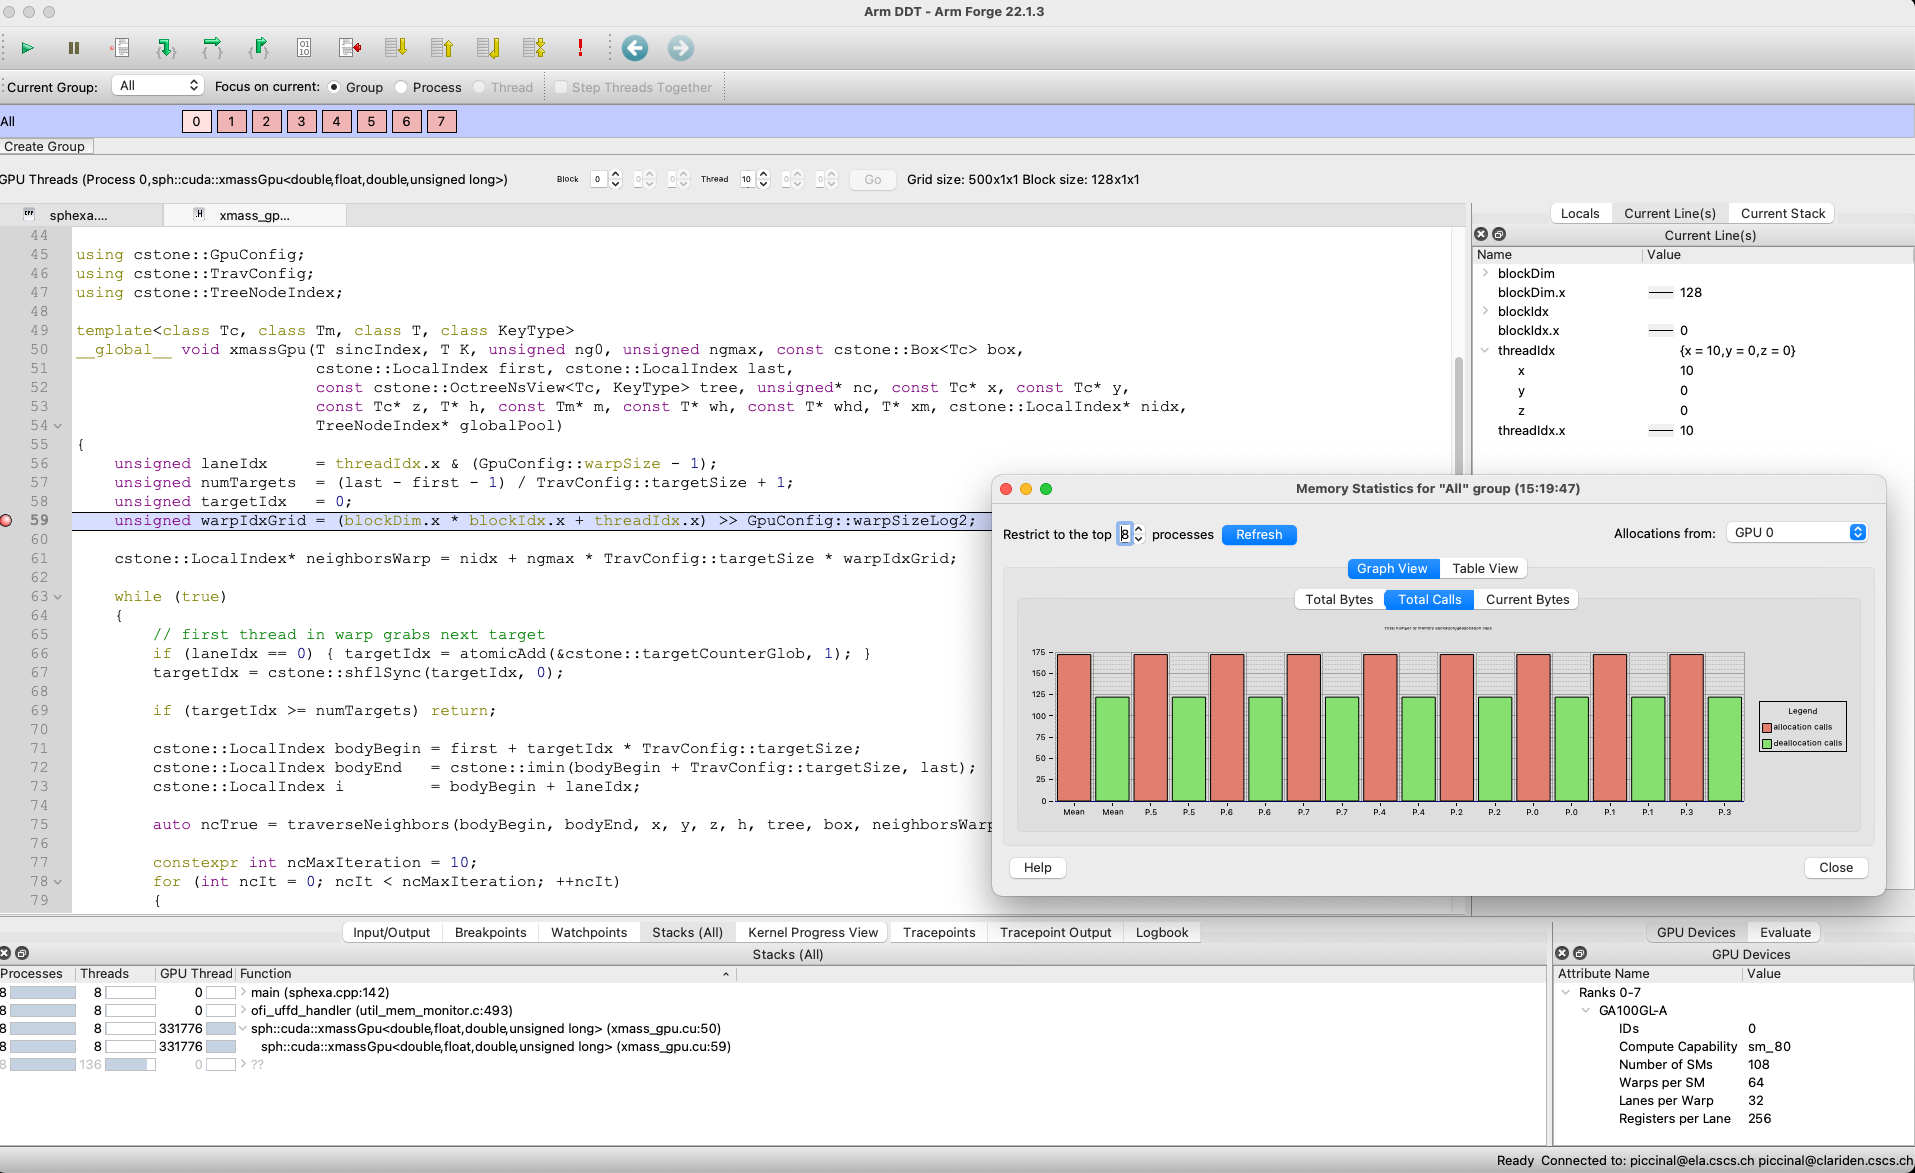
\includegraphics[width=\textwidth]{images/sph-ddt-uenv.png}
    \end{center}
\end{frame}

%-------------------------------------------
\begin{frame}[fragile]{Configuration of mpicc}
\begin{code}{bin/mpicc}
    \begin{lstlisting}[style=talkbash]
prefix="/user-environment/linux-sles15-zen3/gcc-11.3.0/cray-mpich-8.1.18.4-gcc-... long hash ..."
CC="${prefix}/bin/gcc"
$CC ${final_cppflags} ${final_cflags} ${final_ldflags} "${allargs[@]}" -I$includedir -L$libdir -Wl,-rpath,$libdir -lmpi -lmpi_gtl_cuda ${final_libs} \end{lstlisting}
\end{code}

\end{frame}
%-------------------------------------------

%-------------------------------------------
\begin{frame}[fragile]{Objectives}
    We have the following objectives for our software stacks:
    \begin{itemize}
        \item Reproducable from simple recipes:
        \begin{itemize}
            \item versionable with git;
            \item descriptive: what not how.
        \end{itemize}
        \item Separate system-specific configuration from recipe, so that the recipe does not need modification to
        \begin{itemize}
            \item rebuild when a system is updated.
            \item build for different systems.
        \end{itemize}
        %\item Easy roll back.
        %\item Testable.
    \end{itemize}
\end{frame}
%-------------------------------------------


\end{document}
